\newpage
\section{Begriffserklärung}
\label{Begriffe}
Ein Sudoku besteht aus 81 \textit{Feldern} oder \textit{Zellen}. In diese werden die \textit{Ziffern} oder \textit{Zahlen} eingetragen und sie bilden ein Quadrat der Größe 9x9, das \textit{Grid}. Aufgrund dieser Aufteilung hat ein Sudoku 9 \textit{Zeilen} und 9 \textit{Spalten}. Das Grid wird in 9 Unterquadrate geteilt, die jeweils 3x3 Felder groß sind. Diese werden \textit{Blöcke} genannt. Zeilen, Spalten und Blöcke werden unter dem Begriff \textit{Figur} zusammengfasst. Die Nummerierung der Blöcke erfolgt zeilenweise von links oben nach rechts unten.\\
\textit{Vorgaben} sind Zahlen, die schon von Anfang an gegeben sind.\\

\begin{figure}[h]
\begin{center}
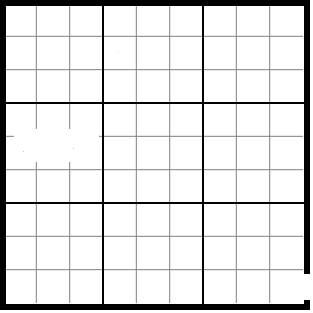
\includegraphics{./img/begriffe.png}
\caption{Sudoku}
\end{center}
\end{figure}

In \textbf{Abbildung 2.2} sieht man im mittleren Block sogenannte \textit{Kandidaten}. Ein Kandidat ist eine Zahl, die in der Zelle noch möglich ist. Jede Zelle hat ihre eigene Liste mit Kandidaten.\\
In der Beschreibung der Lösungstechniken ist es notwendig bestimmte Felder zu betrachten. Hierzu wird eine Abkürzung verwendet, die Zeile und Spalte enthält und somit eine Zelle eindeutig indentifiziert. \textit{z2s3} meint zum Beispiel die Zelle in Zeile 2 und Spalte 3.\\
In der folgenden Abbildung sind die erläuterten Begriffe zum besseren Verständniss eingetragen.\\